 %%%%%%%%%%%%%%%%%%%%%%%%%%%%%%%%%%%%%%%%%%%%%%%%%%%%%%%%%%%%%%%%%%%%%%%%%%%%%%%%
%2345678901234567890123456789012345678901234567890123456789012345678901234567890
%        1         2         3         4         5         6         7         8

\documentclass[conference]{IEEEtran} % Comment this line out
                                                          % if you need a4paper
%\documentclass[a4paper, 10pt, conference]{ieeeconf}      % Use this line for a4
                                                          % paper
\usepackage[ruled]{algorithm2e}
\usepackage{float}
\usepackage{graphicx}
\IEEEoverridecommandlockouts                              % This command is only
                                                          % needed if you want to
                                                          % use the \thanks command
\overrideIEEEmargins
% See the \addtolength command later in the file to balance the column lengths
% on the last page of the document



% The following packages can be found on http:\\www.ctan.org
%\usepackage{graphics} % for pdf, bitmapped graphics files
%\usepackage{epsfig} % for postscript graphics files
%\usepackage{mathptmx} % assumes new font selection scheme installed
%\usepackage{times} % assumes new font selection scheme installed
%\usepackage{amsmath} % assumes amsmath package installed
%\usepackage{amssymb}  % assumes amsmath package installed

\title{\LARGE \bf
PYTHON}

%\author{ \parbox{3 in}{\centering Huibert Kwakernaak*
%         \thanks{*Use the $\backslash$thanks command to put information here}\\
%         Faculty of Electrical Engineering, Mathematics and Computer Science\\
%         University of Twente\\
%         7500 AE Enschede, The Netherlands\\
%         {\tt\small h.kwakernaak@autsubmit.com}}
%         \hspace*{ 0.5 in}
%         \parbox{3 in}{ \centering Pradeep Misra**
%         \thanks{**The footnote marks may be inserted manually}\\
%        Department of Electrical Engineering \\
%         Wright State University\\
%         Dayton, OH 45435, USA\\
%         {\tt\small pmisra@cs.wright.edu}}
%}

\author{
    \IEEEauthorblockN{\Large Yash S. Jain(171080066)}\\
    \IEEEauthorblockA{\IEEEauthorrefmark{1}Dept of Computer Engineering and IT\\
Veermata Jijabai Technological Institute\\
Maharashtra, Mumbai 400019
    \\{Email}:prathmeshbendal@gmail.com}
}


\begin{document}

\maketitle

\thispagestyle{empty}
\pagestyle{empty}


%%%%%%%%%%%%%%%%%%%%%%%%%%%%%%%%%%%%%%%%%%%%%%%%%%%%%%%%%%%%%%%%%%%%%%%%%%%%%%%%
\begin{abstract}

\end{abstract}


%%%%%%%%%%%%%%%%%%%%%%%%%%%%%%%%%%%%%%%%%%%%%%%%%%%%%%%%%%%%%%%%%%%%%%%%%%%%%%%%
\section{Python} \label{ppr12-intro}
Python is an interpreted, high-level, general-purpose programming language. Created by Guido van Rossum and first released in 1991, Python has a design philosophy that emphasizes code readability, notably using significant whitespace. It provides constructs that enable clear programming on both small and large scales.[26] Van Rossum led the language community until stepping down as leader in July 2018.[27][28]

Python features a dynamic type system and automatic memory management. It supports multiple programming paradigms, including object-oriented, imperative, functional and procedural. It also has a comprehensive standard library.[29]

Python interpreters are available for many operating systems. CPython, the reference implementation of Python, is open source software[30] and has a community-based development model, as do nearly all of Python's other implementations. Python and CPython are managed by the non-profit Python Software Foundation. 
\begin{figure}[H]
        \centering
                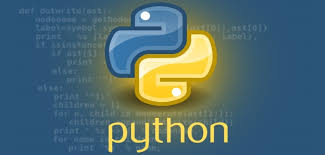
\includegraphics[width=\linewidth]{puthon}
                \caption{python} 
                \label{fig:puthon }
    \end{figure}
    \section{Field-Site Description}  
    
Python was conceived in the late 1980s[31] by Guido van Rossum at Centrum Wiskunde & Informatica (CWI) in the Netherlands as a successor to the ABC language (itself inspired by SETL)[32], capable of exception handling and interfacing with the Amoeba operating system.[7] Its implementation began in December 1989.[33] Van Rossum's long influence on Python is reflected in the title given to him by the Python community: Benevolent Dictator For Life (BDFL) – a post from which he gave himself permanent vacation on July 12, 2018.[34]

Python 2.0 was released on 16 October 2000 with many major new features, including a cycle-detecting garbage collector and support for Unicode.[35]

Python 3.0 was released on 3 December 2008. It was a major revision of the language that is not completely backward-compatible.[36] Many of its major features were backported to Python 2.6.x[37] and 2.7.x version series. Releases of Python 3 include the 2to3 utility, which automates (at least partially) the translation of Python 2 code to Python 3.[38]

Python 2.7's end-of-life date was initially set at 2015 then postponed to 2020 out of concern that a large body of existing code could not easily be forward-ported to Python 3.[39][40] In January 2017, Google announced work on a Python 2.7 to Go transcompiler to improve performance under concurrent workloads.
\begin{figure}[H]
        \centering
                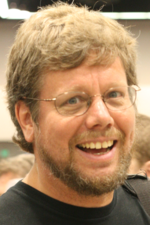
\includegraphics[width=\linewidth]{python}
                \caption{Guido van Rossum } 
                \label{fig:python}
    \end{figure}
    \section{Federal species of concern}
Python uses whitespace indentation, rather than curly brackets or keywords, to delimit blocks. An increase in indentation comes after certain statements; a decrease in indentation signifies the end of the current block.[58] Thus, the program's visual structure accurately represents the program's semantic structure.[1] This feature is also sometimes termed the off-side rule. 
Python's statements include (among others):

    The assignment statement (token '=', the equals sign). This operates differently than in traditional imperative programming languages, and this fundamental mechanism (including the nature of Python's version of variables) illuminates many other features of the language. Assignment in C, e.g., x = 2, translates to "typed variable name x receives a copy of numeric value 2". The (right-hand) value is copied into an allocated storage location for which the (left-hand) variable name is the symbolic address. The memory allocated to the variable is large enough (potentially quite large) for the declared type. In the simplest case of Python assignment, using the same example, x = 2, translates to "(generic) name x receives a reference to a separate, dynamically allocated object of numeric (int) type of value 2." This is termed binding the name to the object. Since the name's storage location doesn't contain the indicated value, it is improper to call it a variable. Names may be subsequently rebound at any time to objects of greatly varying types, including strings, procedures, complex objects with data and methods, etc. Successive assignments of a common value to multiple names, e.g., x = 2; y = 2; z = 2 result in allocating storage to (at most) three names and one numeric object, to which all three names are bound. Since a name is a generic reference holder it is unreasonable to associate a fixed data type with it. However at a given time a name will be bound to some object, which will have a type; thus there is dynamic typing.
    The if statement, which conditionally executes a block of code, along with else and elif (a contraction of else-if).
    The for statement, which iterates over an iterable object, capturing each element to a local variable for use by the attached block.
    The while statement, which executes a block of code as long as its condition is true.
    The try statement, which allows exceptions raised in its attached code block to be caught and handled by except clauses; it also ensures that clean-up code in a finally block will always be run regardless of how the block exits.
    The raise statement, used to raise a specified exception or re-raise a caught exception.
    The class statement, which executes a block of code and attaches its local namespace to a class, for use in object-oriented programming.
    The def statement, which defines a function or method.
    The with statement, from Python 2.5 released on September 2006,[59] which encloses a code block within a context manager (for example, acquiring a lock before the block of code is run and releasing the lock afterwards, or opening a file and then closing it), allowing Resource Acquisition Is Initialization (RAII)-like behavior and replaces a common try/finally idiom.[60]
    The pass statement, which serves as a NOP. It is syntactically needed to create an empty code block.
    The assert statement, used during debugging to check for conditions that ought to apply.
    The yield statement, which returns a value from a generator function. From Python 2.5, yield is also an operator. This form is used to implement coroutines.
    The import statement, which is used to import modules whose functions or variables can be used in the current program. There are three ways of using import: import <module name> [as <alias>] or from <module name> import * or from <module name> import <definition 1> [as <alias 1>], <definition 2> [as <alias 2>], ....
    The print statement was changed to the print() function in Python 3

\begin{figure}[H]
        \centering
                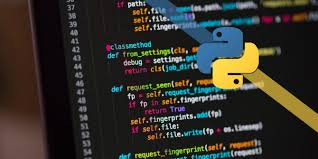
\includegraphics[width=\linewidth]{python1}
                \caption{code} 
                \label{python}
    \end{figure}


\section{LIBRARIES}
Python's large standard library, commonly cited as one of its greatest strengths,[94] provides tools suited to many tasks. For Internet-facing applications, many standard formats and protocols such as MIME and HTTP are supported. It includes modules for creating graphical user interfaces, connecting to relational databases, generating pseudorandom numbers, arithmetic with arbitrary precision decimals,[95] manipulating regular expressions, and unit testing.

Some parts of the standard library are covered by specifications (for example, the Web Server Gateway Interface (WSGI) implementation wsgiref follows PEP 333[96]), but most modules are not. They are specified by their code, internal documentation, and test suites (if supplied). However, because most of the standard library is cross-platform Python code, only a few modules need altering or rewriting for variant implementations.

As of March 2018, the Python Package Index (PyPI), the official repository for third-party Python software, contains over 130,000[97] packages with a wide range of functionality, including:

    Graphical user interfaces
    Web frameworks
    Multimedia
    Databases
    Networking
    Test frameworks
    Automation
    Web scraping[98]
    Documentation
    System administration
    Scientific computing
    Text processing
    Image processing
\section{uses}
Since 2003, Python has consistently ranked in the top ten most popular programming languages in the TIOBE Programming Community Index where, as of December 2018, it is the third most popular language (behind Java, and C).[123] It was selected Programming Language of the Year in 2007, 2010, and 2018.[124]

An empirical study found that scripting languages, such as Python, are more productive than conventional languages, such as C and Java, for programming problems involving string manipulation and search in a dictionary, and determined that memory consumption was often "better than Java and not much worse than C or C++".[125]

Large organizations that use Python include Wikipedia, Google,[126] Yahoo!,[127] CERN,[128] NASA,[129] Facebook,[130] Amazon, Instagram, Spotify[131] and some smaller entities like ILM[132] and ITA.[133] The social news networking site Reddit is written entirely in Python.[134]

Python can serve as a scripting language for web applications, e.g., via mod_wsgi for the Apache web server.[135] With Web Server Gateway Interface, a standard API has evolved to facilitate these applications. Web frameworks like Django, Pylons, Pyramid, TurboGears, web2py, Tornado, Flask, Bottle and Zope support developers in the design and maintenance of complex applications. Pyjs and IronPython can be used to develop the client-side of Ajax-based applications. SQLAlchemy can be used as data mapper to a relational database. Twisted is a framework to program communications between computers, and is used (for example) by Dropbox.

Libraries such as NumPy, SciPy and Matplotlib allow the effective use of Python in scientific computing,[136][137] with specialized libraries such as Biopython and Astropy providing domain-specific functionality. SageMath is a mathematical software with a notebook interface programmable in Python: its library covers many aspects of mathematics, including algebra, combinatorics, numerical mathematics, number theory, and calculus.

Python has been successfully embedded in many software products as a scripting language, including in finite element method software such as Abaqus, 3D parametric modeler like FreeCAD, 3D animation packages such as 3ds Max, Blender, Cinema 4D, Lightwave, Houdini, Maya, modo, MotionBuilder, Softimage, the visual effects compositor Nuke, 2D imaging programs like GIMP,[138] Inkscape, Scribus and Paint Shop Pro,[139] and musical notation programs like scorewriter and capella. GNU Debugger uses Python as a pretty printer to show complex structures such as C++ containers. Esri promotes Python as the best choice for writing scripts in ArcGIS.[140] It has also been used in several video games,[141][142] and has been adopted as first of the three available programming languages in Google App Engine, the other two being Java and Go.[143] Python is also used in algorithmic trading and quantitative finance.[144] Python can also be implemented in APIs of online brokerages that run on other languages by using wrappers.[145]

Python is commonly used in artificial intelligence projects with the help of libraries like TensorFlow, Keras and Scikit-learn.[146][147][148][149] As a scripting language with modular architecture, simple syntax and rich text processing tools, Python is often used for natural language processing.[150]

Many operating systems include Python as a standard component. It ships with most Linux distributions, AmigaOS 4, FreeBSD, NetBSD, OpenBSD and macOS, and can be used from the command line (terminal). Many Linux distributions use installers written in Python: Ubuntu uses the Ubiquity installer, while Red Hat Linux and Fedora use the Anaconda installer. Gentoo Linux uses Python in its package management system, Portage.

Python is used extensively in the information security industry, including in exploit development.[151][152]

Most of the Sugar software for the One Laptop per Child XO, now developed at Sugar Labs, is written in Python.[153] The Raspberry Pi single-board computer project has adopted Python as its main user-programming language. Since 2003, Python has consistently ranked in the top ten most popular programming languages in the TIOBE Programming Community Index where, as of December 2018, it is the third most popular language (behind Java, and C).[123] It was selected Programming Language of the Year in 2007, 2010, and 2018.[124]

An empirical study found that scripting languages, such as Python, are more productive than conventional languages, such as C and Java, for programming problems involving string manipulation and search in a dictionary, and determined that memory consumption was often "better than Java and not much worse than C or C++".[125]

Large organizations that use Python include Wikipedia, Google,[126] Yahoo!,[127] CERN,[128] NASA,[129] Facebook,[130] Amazon, Instagram, Spotify[131] and some smaller entities like ILM[132] and ITA.[133] The social news networking site Reddit is written entirely in Python.[134]

Python can serve as a scripting language for web applications, e.g., via mod_wsgi for the Apache web server.[135] With Web Server Gateway Interface, a standard API has evolved to facilitate these applications. Web frameworks like Django, Pylons, Pyramid, TurboGears, web2py, Tornado, Flask, Bottle and Zope support developers in the design and maintenance of complex applications. Pyjs and IronPython can be used to develop the client-side of Ajax-based applications. SQLAlchemy can be used as data mapper to a relational database. Twisted is a framework to program communications between computers, and is used (for example) by Dropbox.

Libraries such as NumPy, SciPy and Matplotlib allow the effective use of Python in scientific computing,[136][137] with specialized libraries such as Biopython and Astropy providing domain-specific functionality. SageMath is a mathematical software with a notebook interface programmable in Python: its library covers many aspects of mathematics, including algebra, combinatorics, numerical mathematics, number theory, and calculus.

Python has been successfully embedded in many software products as a scripting language, including in finite element method software such as Abaqus, 3D parametric modeler like FreeCAD, 3D animation packages such as 3ds Max, Blender, Cinema 4D, Lightwave, Houdini, Maya, modo, MotionBuilder, Softimage, the visual effects compositor Nuke, 2D imaging programs like GIMP,[138] Inkscape, Scribus and Paint Shop Pro,[139] and musical notation programs like scorewriter and capella. GNU Debugger uses Python as a pretty printer to show complex structures such as C++ containers. Esri promotes Python as the best choice for writing scripts in ArcGIS.[140] It has also been used in several video games,[141][142] and has been adopted as first of the three available programming languages in Google App Engine, the other two being Java and Go.[143] Python is also used in algorithmic trading and quantitative finance.[144] Python can also be implemented in APIs of online brokerages that run on other languages by using wrappers.[145]

Python is commonly used in artificial intelligence projects with the help of libraries like TensorFlow, Keras and Scikit-learn.[146][147][148][149] As a scripting language with modular architecture, simple syntax and rich text processing tools, Python is often used for natural language processing.[150]

Many operating systems include Python as a standard component. It ships with most Linux distributions, AmigaOS 4, FreeBSD, NetBSD, OpenBSD and macOS, and can be used from the command line (terminal). Many Linux distributions use installers written in Python: Ubuntu uses the Ubiquity installer, while Red Hat Linux and Fedora use the Anaconda installer. Gentoo Linux uses Python in its package management system, Portage.

Python is used extensively in the information security industry, including in exploit development.[151][152]

Most of the Sugar software for the One Laptop per Child XO, now developed at Sugar Labs, is written in Python.[153] The Raspberry Pi single-board computer project has adopted Python as its main user-programming language. 
\bibliographystyle{unsrt}
\bibliography{References/Refer}
\end{document}

